\documentclass[../DefinizioneDiProdotto.tex]{subfiles}

\begin{document}

\section{Descrizione architetturale}

	\subsection{Design pattern}

		\subsubsection{Architetturali}
		Durante la progettazione si è deciso di adattare diversi \gl{design pattern architetturali}, difatti secondo le nostre esigenze, non era possibile adottarne uno identico per tutta l'architettura.
		E' stato quindi deciso l'uso del pattern MVC per la porzione logica identificata come Front-End, e una gestione ad eventi, servizio appositamente offerto da Amazon, per la sezione identificata come Back-End.
		Per la risoluzione delle dipendenze, è stato infine utilizzato il pattern Dependency Injection, utilizzato da Angular.
			\paragraph{MVC}\mbox{}
			\begin{addmargin}[1em]{2em}% 1em left, 2em right
				\textbf{Scopo}: il Model è il livello più basso del pattern ed è responsabile della gestione dei dati utili all'applicazione. La View si occupa di visualizzare le informazioni, presenti nel Model, all'utente. Il Controller invece si occupa del controllo tra le interazioni tra Model e View.\\
				\textbf{Utilizzo}: il design pattern MVC (Model View Controller) viene utilizzato a livello di componentistica, ognuna delle quali contiene un Model, una View ed un Controller.\\
				\textbf{Motivo}: questa scelta è stata dettata dall'impiego di AngularJS per la realizzazione del front-end, della console amministrativa e della schermata per l'ospite, che utilizzando un pattern MVC ci ha influenzati. Un'altra motivazione è fornita dall'utilizzo delle REST API, e dalla possibilità di sfruttare gli oggetti da parte di AngularJS e nella versione NodeJS da noi utilizzata, in questo modo possiamo trattare mediante interfaccia REST lo stesso oggetto che fa da Model, come oggetto nella parte di back-end. Il Controller si interfaccia verso le API da un'apposita classe chiamate Service.\\
Per facilitare la comprensione di quanto appena descritto, viene fornito una schema riportante la struttura MVC adottata.
			\end{addmargin}
			\newpage
			\begin{figure}[!h]
			\centering
				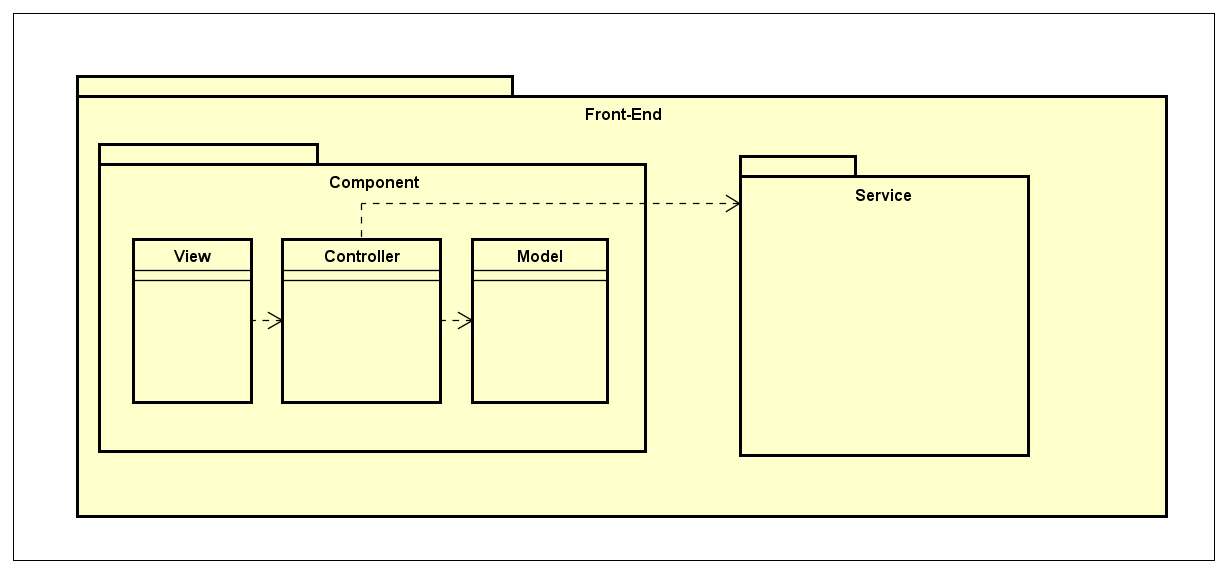
\includegraphics[width=\textwidth]{Architettura/MVC.png}
				\caption{Schema MVC}
			\end{figure}

			\paragraph{Event-Driven}\mbox{}
			\begin{addmargin}[1em]{2em}% 1em left, 2em right
				\textbf{Scopo}:	un evento può essere formato da due parti, l'intestazione dell'evento ed il suo corpo. Il primo include per informazioni come nome, \gl{timestamp} dell'evento e il suo tipo. Il corpo invece fornisce i dettagli del cambiamento di stato.\\
				\textbf{Utilizzo}: gestione ottimizzata di AWS Lambda mediante AWS SNS .\\
				\textbf{Motivo}: questa scelta è dovuta principalmente al metodo di fatturazione di Amazon AWS. Facendo così, una volta lanciato l'evento, la lambda function si sospende e non consuma tempo di esecuzione per la richiesta \gl{HTTP}. Inoltre grazie al \gl{precaching}, potendo suddividere i moduli più complessi in più lambda si riduce la memoria utilizzata per funzione ed il tempo di caricamento.
			\end{addmargin}

			\paragraph{REST API}\mbox{}
			\begin{addmargin}[1em]{2em}% 1em left, 2em right
				\textbf{Scopo}: REST API (REpresentational State Transfer Application Programming Interface) consiste in sei vincoli da rispettare:
					\begin{itemize}
						\item \textbf{Client-Server}: richiede la separazione tra l'interfaccia utente dai dati da archiviare, così da migliorare la portabilità dell'interfaccia tra diverse piattaforme e la scalabilità, semplificando i componenti server. Così facendo si possono sviluppare i componenti indipendentemente;
						\item \textbf{Stateless}: la comunicazione client-server è vincolata dall'assenza di una memorizzazione, nel server, del contesto. Ogni chiamata, non possiede nessuna memoria delle precedenti avvenute, questo non implica però che, al di fuori della chiamata, ci siano dei token di riconoscimento appositi;
						\item \textbf{Cacheable}:  i client possono fare \gl{caching} delle risposte. Le risposte devono in ogni modo definirsi implicitamente o esplicitamente cacheable o no, in modo da prevenire che i client possano riusare stati datati o dati errati. Una gestione ben fatta della cache può ridurre, o parzialmente eliminare, le comunicazioni client-server, migliorando scalabilità e performance;
						\item \textbf{Layered system}: un client non può dire se è connesso direttamente ad un server di livello più basso o intermedio. I server intermedi possono migliorare la scalabilità del sistema con \gl{load-balancing} o con \gl{cache distribuite}. Possono esserci \gl{layer} intermedi per offrire inoltre politiche di sicurezza;
						\item \textbf{Code on demand}:  i server possono temporaneamente estendere o personalizzare le funzionalità del client trasferendo del codice eseguibile. Ad esempio questo può includere componenti compilati come \gl{Applet Java} o linguaggi di scripting client-side come JavaScript. "Code on demand" è l'unico vincolo opzionale per la definizione di un'architettura REST;
						\item \textbf{Uniform interface}: un'interfaccia di comunicazione omogenea tra client e server permette di semplificare e disaccoppiare l'architettura, la quale si può evolvere separatamente.
					\end{itemize}.\\
				\textbf{Utilizzo}: viene utilizzato nell'interfaccia tra Front-End e Back-End.\\
				\textbf{Motivo}: questa scelta è dovuta alla larga diffusione di questo metodo per la gestione di chiamate HTTP/HTTPS, che lo rende ormai standard, e per la semplicità di implementazione con il meccanismo lambda di Amazon che ne fornisce un apposito servizio (AWS APIGateway) interfacciato con \gl{SWAGGER}.

			\end{addmargin}
			\begin{figure}[!h]
			\centering
				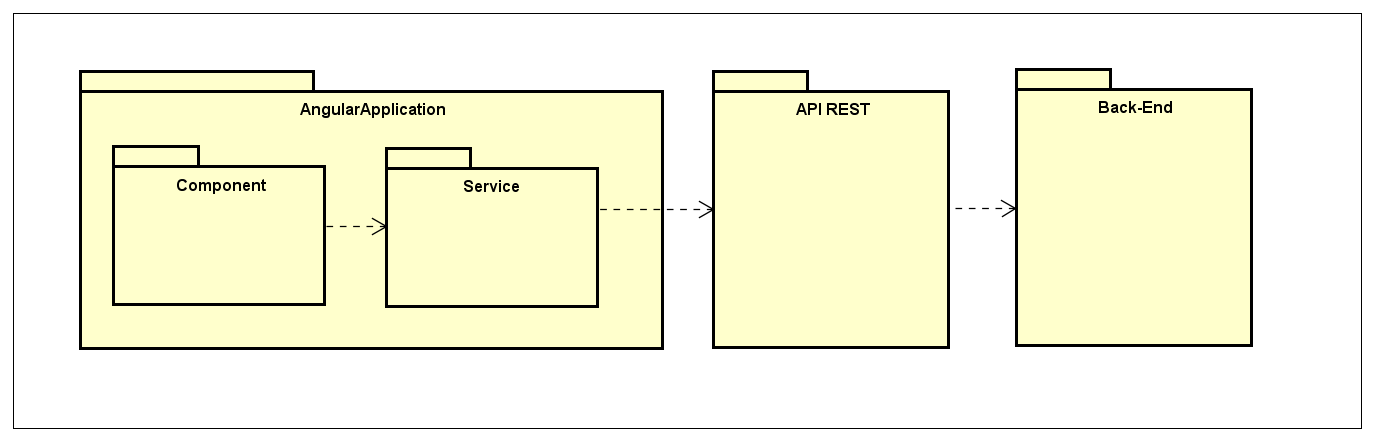
\includegraphics[width=\textwidth]{Architettura/API-Rest.png}
				\caption{Schema REST API}
			\end{figure}

			\paragraph{Dependency Injection}\mbox{}
			\begin{addmargin}[1em]{2em}% 1em left, 2em right
				\textbf{Scopo}: semplificare lo sviluppo e rendere più testabile un software di grandi dimensioni. Separa il codice della componente dal codice che si occupa di risolvere le dipendenze con altre componenti.\\
				\textbf{Utilizzo}: Dependency Injection è parte integrante di AngularJS e viene utilizzato nel Front-End ogni volta che una funzione ha bisogno di richiamare una funzionalità esterna.\\
				\textbf{Motivo}: con questo pattern è possibile esprimere le dipendenze in modo dichiarativo e utilizzare un oggetto contenitore per risolverle dinamicamente a \gl{runtime}. In questo modo è possibile scegliere anche quale componente iniettare in base allo stato del programma.
			\end{addmargin}

		\subsubsection{Comportamentali}
		Viene adottato un solo \gl{design pattern comportamentale} nell'architettura, l'Observer, per sincronizzare i vari oggetti dipendenti tra loro.

			\paragraph{Observer}\mbox{}
			\begin{addmargin}[1em]{2em}% 1em left, 2em right
				\textbf{Scopo}: definisce una dipendenza "1..n" fra oggetti, riflettendo la modifica di un oggetto su quelli ad esso dipendenti.\\
				\textbf{Utilizzo}: viene utilizzato tra i \gl{services} e i \gl{component} del Front-End.\\
				\textbf{Motivo}: in alcuni casi è necessario tenere sincronizzati vari oggetti e, nel caso un oggetto venga modificato, avere la possibilità di riflettere il cambiamento sugli oggetti dipendenti.
			\end{addmargin}


	\subsection{Architettura generale}
		\subsubsection{Schema architettura generale}
		\begin{figure}[!h]
			\centering
			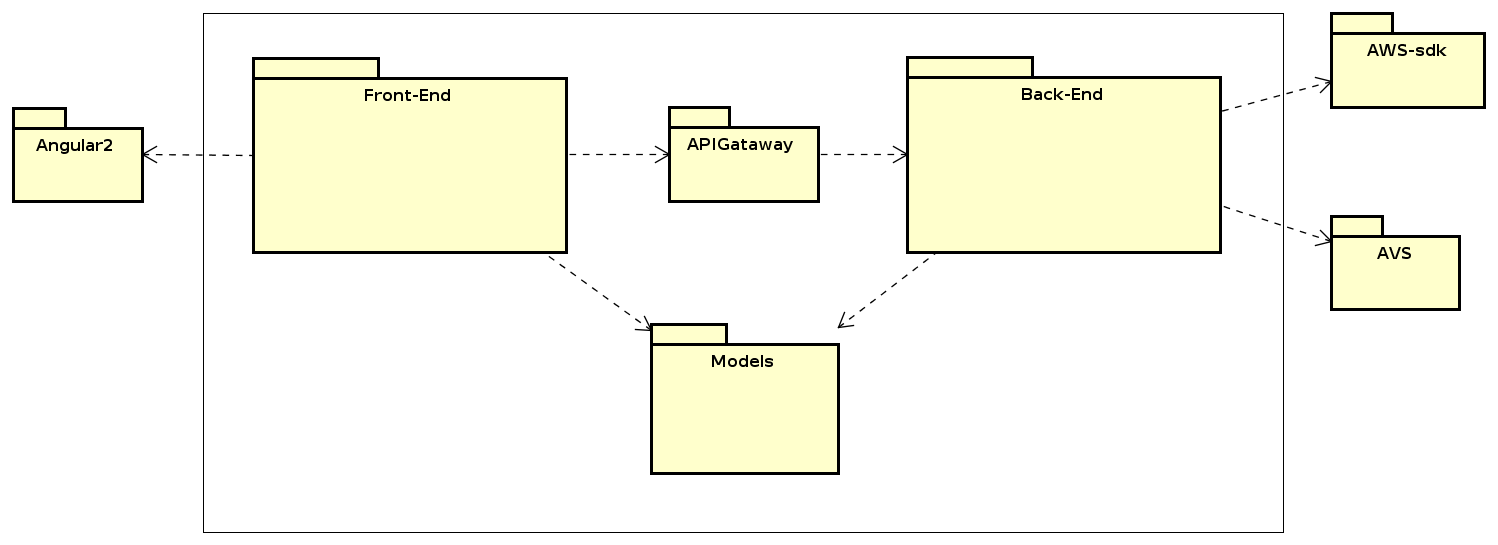
\includegraphics[width=\textwidth]{Architettura/AltoLivello.png}
			\caption{Schema architettura generale}
		\end{figure}

		\subsubsection{Descrizione}
		Nell'esposizione dell'architettura dell'applicazione si procederà con un approccio \gl{top-down}, descrivendola dal generico al particolare. Si inizia quindi dalla descrizione dei package e dei componenti, per poi descrivere nel dettaglio le singole classi, specificando per ognuna il tipo, l'obiettivo, la funzione, relazioni in ingresso e uscita e i metodi e attributi contenuti. Successivamente verranno riportati i diagrammi di sequenza da quelli più generali a quelli delle singole chiamate API, il tutto seguendo il formalismo del linguaggio UML 2.0.

		\subsubsection{Suddivisione logica}
		La prima suddivisione riguarda il Front-End ed il Back-End con al centro un package, ovvero l'AWS APIGateway, senza però una precisa implementazione vista la sua necessita di essere configurato tramite SWAGGER. È stata implementata una separazione tra GuestHome e i suoi Services, e la parte di amministrazione con i relativi Services. Lo stesso è stato fatto per la parte del Back-End. Ad esempio, il package del back-end LambdaSkill contiene tutti i moduli relativi alla comunicazione con l'ospite ed hanno in comune solo i moduli che contengono le specifiche dei singoli oggetti.

		\newpage
		\subsubsection{Architettura Front-end}
		\begin{figure}[h]
			\centering
			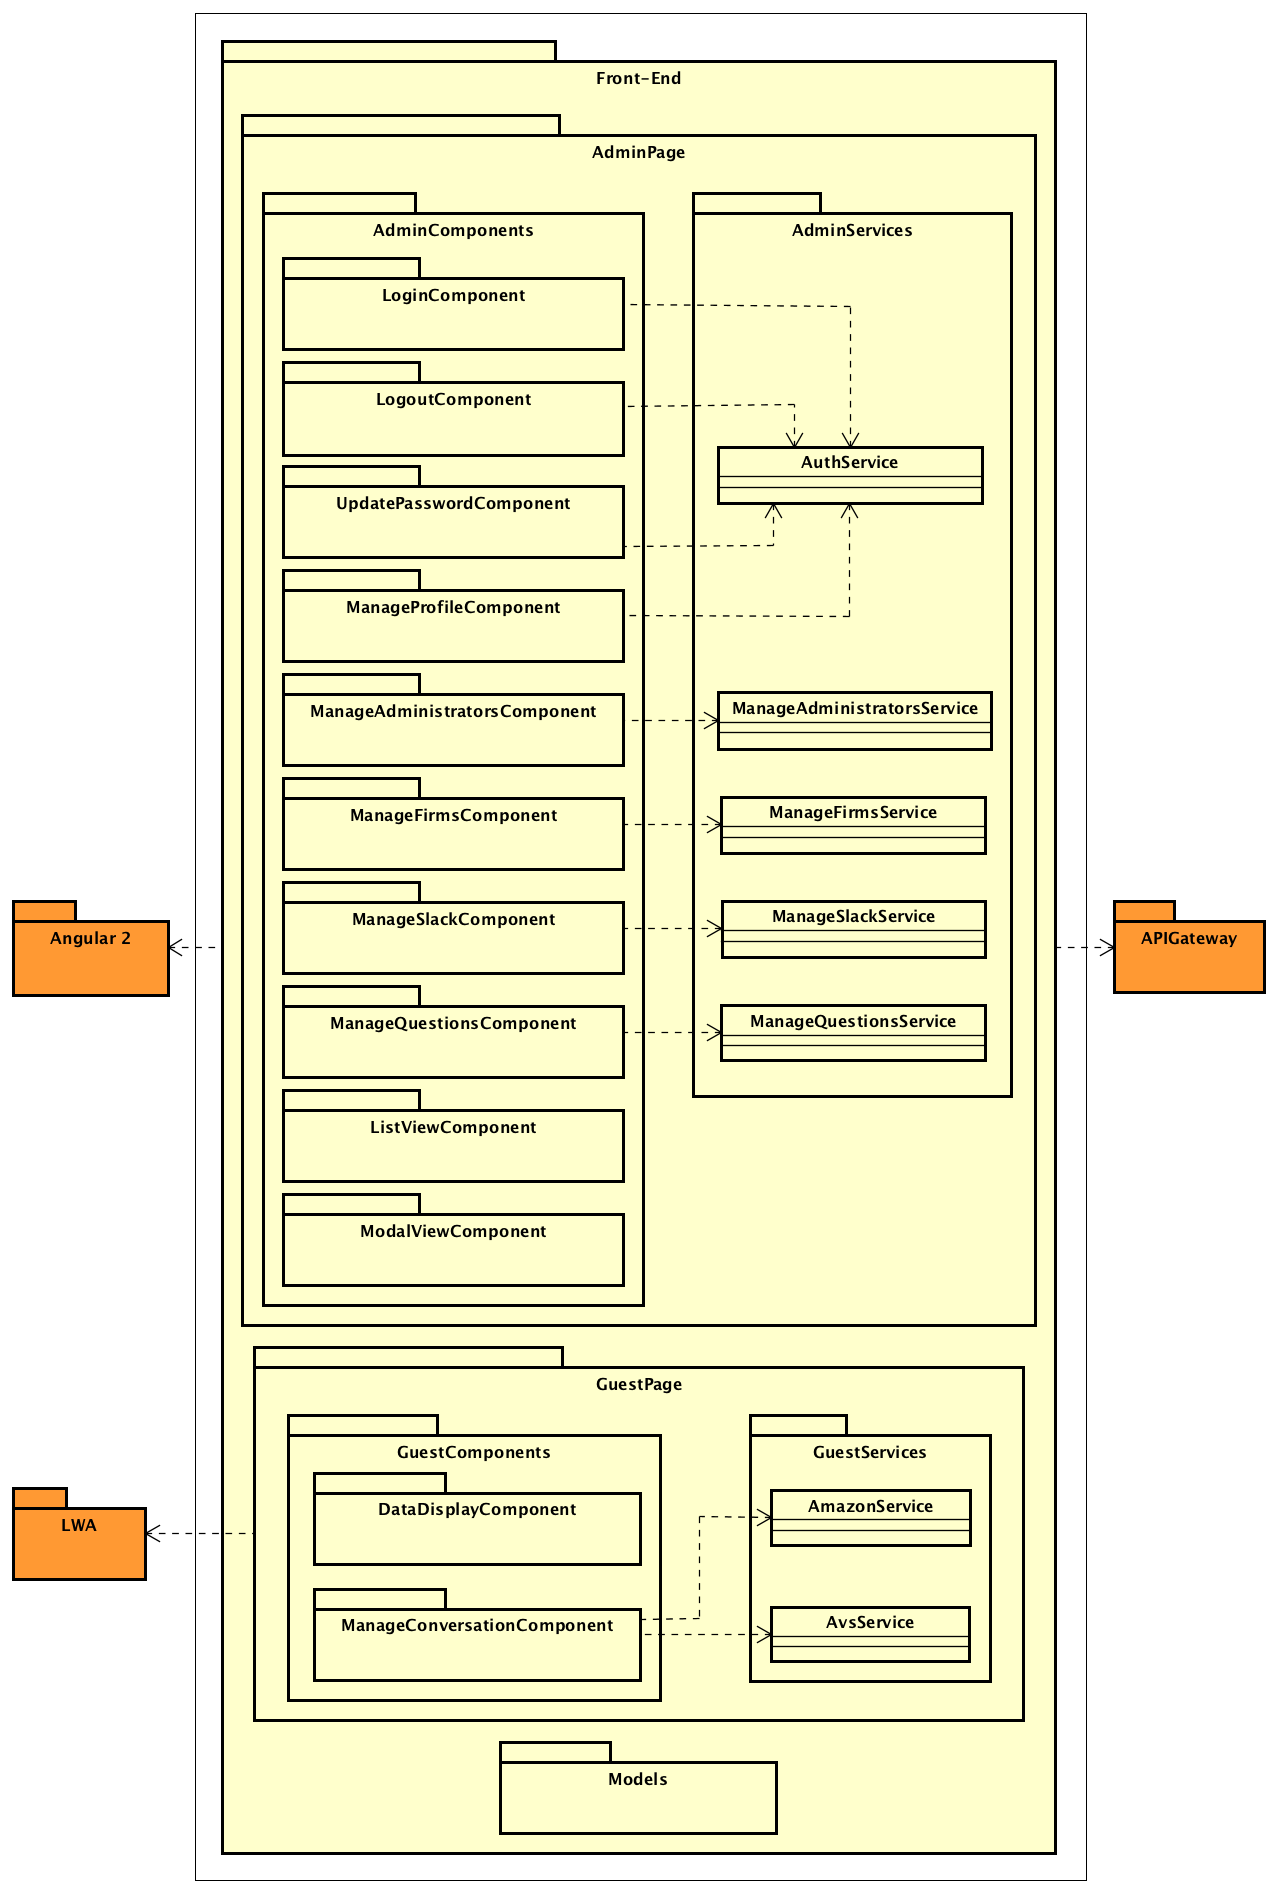
\includegraphics[width=\textwidth]{Architettura/Front-end.png}
			\caption{Schema architettura Front-End}
		\end{figure}

		\paragraph{Descrizione}	La parte del Front-End è sviluppata in AngularJS e ne rispecchia il pattern di sviluppo: ogni componente (ogni package rappresenta un Model-View-Controller) è immerso nella pagina. Di seguito è disponibile una lista delle \gl{route} delle pagine per i relativi tracciamenti per comprendere al meglio quando i vari componenti vengono attivati. \\ \\

			\begin{longtable}[c] { >{\centering\arraybackslash}p{5cm} >{\centering\arraybackslash}p{5cm} }
				\toprule
				{\textbf{Componente}} & {\textbf{Route}} \\
				\midrule
				Login &  /admin/login \\
		 		\addlinespace[0.3em]
				\midrule
				UpdatePassword & /admin/updatePassword   \\
		 		\addlinespace[0.3em]
				\midrule
				ManageGuests &  /admin/manageGuest \\
		 		\addlinespace[0.3em]
				\midrule
				ManageAdministrators &  /admin/manageAdmins \\
		 		\addlinespace[0.3em]
				\midrule
				ManageSlack &  /admin/manageSlack \\
		 		\addlinespace[0.3em]
				\midrule
				ManageQuestions & /admin/manageQuestions  \\
		 		\addlinespace[0.3em]
				\midrule
				ManageProfile &  /admin/manageProfile \\
		 		\addlinespace[0.3em]
				\midrule
				StartStop &  /guestHome \\
		 		\addlinespace[0.3em]
				\midrule
				DataDisplay &  /guestHome \\
		 		\addlinespace[0.3em]
				\midrule
				Conversation &  /guestHome \\
		 		\addlinespace[0.3em]
				\bottomrule
				\caption{Tracciamento Component-Route AngularJS}
			\end{longtable}

		\newpage
		\subsubsection{Architettura Back-End}
		\begin{figure}[!h]
			\centering
			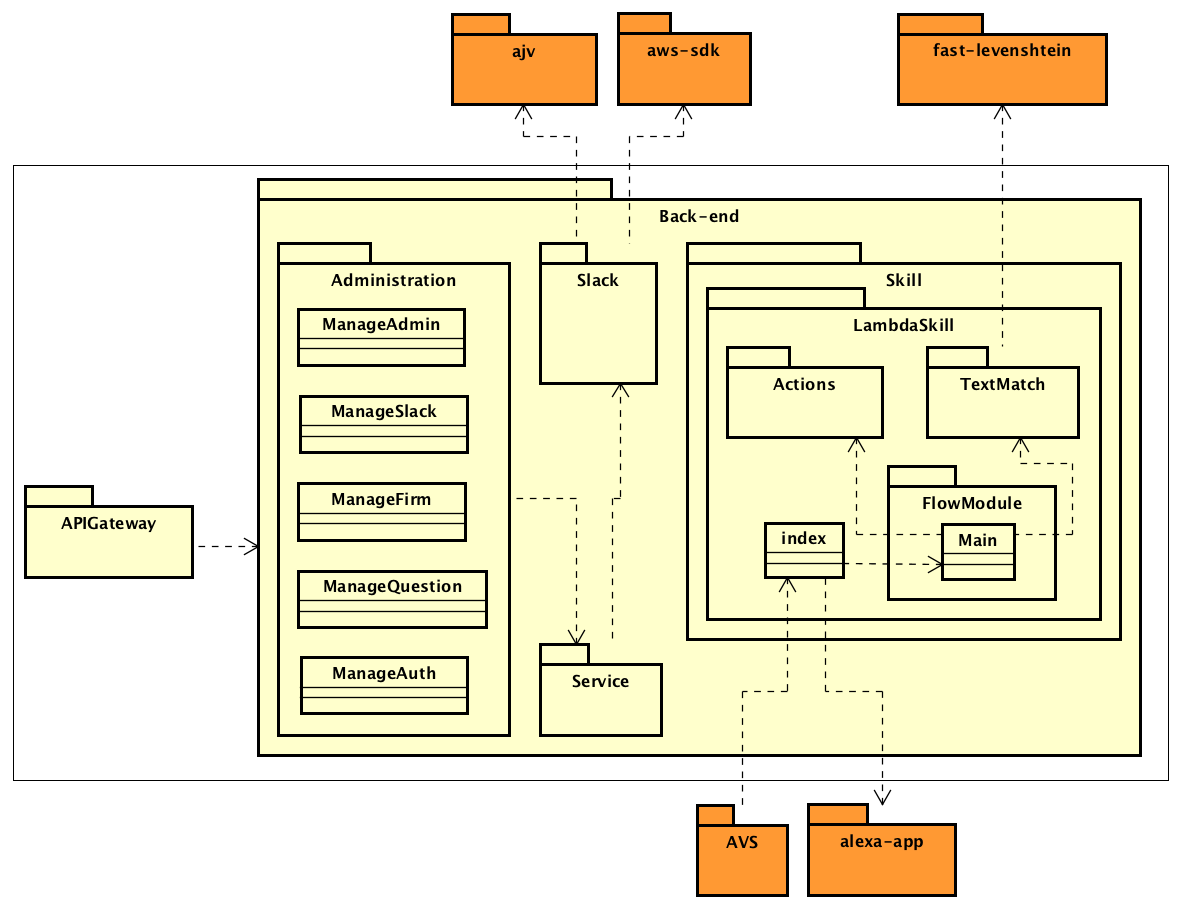
\includegraphics[width=\textwidth]{Architettura/Back-end.png}
			\caption{Schema architettura Back-End}
		\end{figure}

		\paragraph{Descrizione}

		Nel Back-End sono stati progettate separatamente le componenti che interagiscono con l'API Gateway per l'amministrazione e quelle che invece riguardano GuestHome. Il punto di dipendenza verso l'accesso al database, a Slack e con l'altra componente riguarda esclusivamente il package Service, che fornisce i metodi per la gestione , il salvataggio e il reperimento degli oggetti. Il package LambdaSkill gestisce l'evento ricevuto dalla Skill di Alexa e il flusso delle domande a porre.

	\newpage
	\subsection{Servizi REST}
Come è stato possibile capire dalla sezione sulle REST API scritta precedentemente, per
gestire l'interazione tra Back-End e Front-End vengono utilizzati dei servizi REST. Nelle
REST API viene passato l'intero oggetto, anziché solo i parametri da modificare, questo
per avere un'attività di codifica più semplice e per facilitare eventuali modifiche, con il
compromesso però di avere un maggior utilizzo di risorse riguardante al traffico di sistema.\\
L'elenco dei servizi REST usati e dei pattern viene riportato nelle seguenti tabelle suddivise per package e per classe.

	\subsubsection{ServicesAmministrazione}
	\begin{longtable}[c] { >{\centering\arraybackslash}p{3cm} >{\centering\arraybackslash}p{6cm}}
				\toprule
				\centerline{\textbf{Funzioni}} & \centerline{\textbf{REST}} \\
				\midrule
				getAdmins &  GET: lista amministratori \\
		 		\addlinespace[0.3em]
				\midrule
				\addlinespace[0.3em]
				addAdmin & POST: aggiungi amministratore \\
		 		\addlinespace[0.3em]
				\midrule
				\addlinespace[0.3em]
				updateAdmin & PUT: modifica admin \\
		 		\addlinespace[0.3em]
				\midrule
				\addlinespace[0.3em]
				deleteAdmin & DELETE: cancella admin \\

				\bottomrule
				\caption{ManageAdministrators}
		\end{longtable}

		\begin{longtable}[c] { >{\centering\arraybackslash}p{4cm} >{\centering\arraybackslash}p{6cm}}
				\toprule
				\centerline{\textbf{Funzioni}} & \centerline{\textbf{REST}} \\
				\midrule
				getInterlocutors &  GET: lista interlocutori \\
		 		\addlinespace[0.3em]
				\midrule
				\addlinespace[0.3em]
				getDefaultInterlocutors & GET: lista interlocutori default \\
		 		\addlinespace[0.3em]
				\midrule
				\addlinespace[0.3em]
				addToDefault & POST: aggiungi interlocutore di default \\
		 		\addlinespace[0.3em]
				\midrule
				\addlinespace[0.3em]
				removeToDefault & DELETE: rimuovi interlocutore di default \\

				\bottomrule
				\caption{ManageSlack}
		\end{longtable}

		\newpage
		\begin{longtable}[c] { >{\centering\arraybackslash}p{3cm} >{\centering\arraybackslash}p{6cm}}
				\toprule
				\centerline{\textbf{Funzioni}} & \centerline{\textbf{REST}} \\
				\midrule
				getFirms &  GET: lista delle aziende \\
		 		\addlinespace[0.3em]
				\midrule
				\addlinespace[0.3em]
				updateFirm & PUT: update azienda (con guest dentro) \\
		 		\addlinespace[0.3em]
				\midrule
				\addlinespace[0.3em]
				updateFirm & GET: conversazione del guest \\

				\bottomrule
				\caption{ManageFirm}
		\end{longtable}

		\begin{longtable}[c] { >{\centering\arraybackslash}p{3cm} >{\centering\arraybackslash}p{6cm}}
				\toprule
				\centerline{\textbf{Funzioni}} & \centerline{\textbf{REST}} \\
				\midrule
				login &  GET: verifica dati di login inseriti \\
		 		\addlinespace[0.3em]
				\midrule
				\addlinespace[0.3em]
				verifyLogin & GET: verifica se token passato è corretto \\
		 		\addlinespace[0.3em]
				\midrule
				\addlinespace[0.3em]
				logout & PUT: rimozione token \\
		 		\addlinespace[0.3em]
				\midrule
				\addlinespace[0.3em]
				sendEmail & GET: invia mail recupero password \\

				\bottomrule
				\caption{ManageAuth}
		\end{longtable}

		\begin{longtable}[c] { >{\centering\arraybackslash}p{3cm} >{\centering\arraybackslash}p{6cm}}
				\toprule
				\centerline{\textbf{Funzioni}} & \centerline{\textbf{REST}} \\
				\midrule
				getQuestions &  GET: lista domande \\
		 		\addlinespace[0.3em]
				\midrule
				\addlinespace[0.3em]
				getActions & GET: lista azioni \\
		 		\addlinespace[0.3em]
				\midrule
				\addlinespace[0.3em]
				updateQuestion & PUT: modifica una domanda \\
		 		\addlinespace[0.3em]
				\midrule
				\addlinespace[0.3em]
				deleteQuestion & DELETE: elimina una domanda \\
				\addlinespace[0.3em]
				\midrule
				\addlinespace[0.3em]
				addQuestion & POST: aggiunge una domanda \\

				\bottomrule
				\caption{ManageQuestions}
		\end{longtable}

	\newpage
	\subsubsection{InteractionService}
	\begin{longtable}[c] { >{\centering\arraybackslash}p{3cm} >{\centering\arraybackslash}p{6cm}}
				\toprule
				\centerline{\textbf{Funzioni}} & \centerline{\textbf{REST}} \\
				\midrule
				enable &  POST: attivazione sessione (creare conversazione) \\
		 		\addlinespace[0.3em]
				\midrule
				\addlinespace[0.3em]
				disable & DELETE: rimozione della sessione \\
		 		\addlinespace[0.3em]
				\midrule
				\addlinespace[0.3em]
				call & GET: chiama skill \\
		 		\addlinespace[0.3em]
				\midrule
				\addlinespace[0.3em]
				getText & GET: testo risposta precedente \\

				\bottomrule
				\caption{Interaction}
		\end{longtable}

	\subsection{Struttura database}
	Di seguito viene riportato la struttura del database suddivisa per oggetti di collezione.
		\subsubsection{Question}
		Question contiene le informazioni di una domanda.
		\begin{lstlisting}[language=json,firstnumber=1]
{
  "id": (int),
  "baseText": (String),
  "recurrentText": (String),
  "answers": [{
     "text": (String),
     "id_nextQuestion": (int),
     "action": {
        "id": (String),
        "text": (String)
      }
   }]
}
		\end{lstlisting}

		\subsubsection{Firm}
		Serve per contenere le informazioni di un'azienda.
		\begin{lstlisting}[language=json,firstnumber=1]
{
  "id": (int)
  "name": (String),
  "guests": [{
     "id": (int)
     "name": (String)
   }]
}
		\end{lstlisting}

		\subsubsection{Admin}
		Questo modello contiene le informazioni riguardanti gli amministratori.
		\begin{lstlisting}[language=json,firstnumber=1]
{
  "id": (int),
  "username": (String),
  "email": (String),
  "password": (String)
}
		\end{lstlisting}

		\subsubsection{Interlocutor}
		Interlocutor contiene le informazioni riguardanti gli interlocutori per i canali Slack.
		\begin{lstlisting}[language=json,firstnumber=1]
{
  "id": (int),
  "id_slack": (String),
  "name": (String),
  "joinChannel": (boolean)
}
		\end{lstlisting}

		\subsubsection{Conversation}
		Conversation è un modello usato per contenere le informazioni sulle conversazioni fatte tra l'ospite e l'assistente virtuale.
		\begin{lstlisting}[language=json,firstnumber=1]
{
  "id_session": (int),
  "log": [{
     "id_guest": (int),
      "question": (String),
      "answer": (String),
     "date": (String)
   }]
}
		\end{lstlisting}

	\subsection{Pacchetti di interazione}
	Per facilitare l'interazione tra i componenti del sistema sono stati inseriti dei \gl{trame}, ovvero dei pacchetti \gl{JSON} per permettere la comunicazione tra funzioni e tra moduli del sistema.
	\begin{itemize}
		\item \textbf{API trame}: viene utilizzato per la risposta alle chiamate in tutto il Back-End e contiene le informazioni per la gestione degli errori e l'oggetto che la funzione avrebbe dovuto ritornare. Questo torna particolarmente utile, per ridurre la complessità della gestione degli errori, tra lambda function con APIGateway e APIGateway con Service, nella parte di Front-End.\\
		Viene ora riportato il pacchetto JSON per quanto riguarda l'API trame.
		\begin{lstlisting}[language=json,firstnumber=1]
{
  Error: (boolean),
  TypeError: (string),
  Object: (JSONObject)
}
		\end{lstlisting}

		\item \textbf{Admin trame}: viene utilizzato per incapsulare l'oggetto passato alla chiamata HTTP e il token di autenticazione, per quelle chiamate ai moduli che richiedono autorizzazioni a livello di utente per ricevere risposta. Riduce il numero di parametri richiesti alle funzioni e riduce il numero di parametri dell'interfaccia che l'APIGateway può vedere. L'utilizzo è ristretto ai service del Front-End riguardanti l'amministrazione e alla relativa controparte nel Back-End.\\
		Viene ora riportato il pacchetto JSON per quanto riguarda l'Admin trame.
		\begin{lstlisting}[language=json,firstnumber=1]
{
  Error: (boolean),
  TypeError: (string),
  Object: (JSONObject)
}
		\end{lstlisting}
	\end{itemize}

	\subsection{Semantica rappresentativa}
	In JavaScript non esiste una reale implementazione dei package. Il loro utilizzo è stato quindi dichiarato per rendere una chiara suddivisione logica dei vari componenti.
	Alcuni di questi però, nella sezione Back-End, potranno diventare dei moduli NodeJS per
	semplificare l'utilizzo in AWS Lambda.
	In JavaScript, con la specifica \gl{ECMA script 6} è stato reso possibile strutturare gli oggetti
	in classi. Le versioni di AngularJS e NodeJS che andremo ad utilizzare ne permetteranno
	quindi l'utilizzo.
	Per rendere chiaro dove le unità logiche rappresentate nella nostra architettura verranno
	rappresentate come effettive classi, e quali invece sono solo delle unità logiche, abbiamo
	generato due tabelle che indicano questa suddivisione.
	Di seguito sono riportate due tabelle, la prima per le classi concrete che contengono quindi	i campi dati e le implementazioni di tutti i metodi e la seconda invece contiene quelle rappresentative.
			\begin{longtable}[c] { >{\centering\arraybackslash}p{13cm} }
				\toprule
				\centerline{\textbf{Nome}} \\
				\midrule
				Front-End::AdministrationView::AdminService::Authentication \\
				\addlinespace[0.3em]
				\midrule
				\addlinespace[0.3em]
				Front-End::AdministrationView::AdminService::ManageAdminstrators \\
				\addlinespace[0.3em]
				\midrule
				\addlinespace[0.3em]
				Front-End::AdministrationView::AdminService::ManageGuest \\
				\addlinespace[0.3em]
				\midrule
				\addlinespace[0.3em]
				Front-End::AdministrationView::AdminService::ManageSlack \\
				\addlinespace[0.3em]
				\midrule
				\addlinespace[0.3em]
				Front-End::AdministrationView::AdminService::ManageQuestions \\
				\addlinespace[0.3em]
				\midrule
				\addlinespace[0.3em]
				Front-End::AdministrationView::AdminComponents::Login::LoginController \\
				\addlinespace[0.3em]
				\midrule
				\addlinespace[0.3em]
				Front-End::AdministrationView::AdminComponents::ManageProfile::\\ManageProfileController \\
				\addlinespace[0.3em]
				\midrule
				\addlinespace[0.3em]
				Front-End::AdministrationView::AdminComponents::UpdatePassword::\\UpdatePasswordController \\
				\addlinespace[0.3em]
				\midrule
				\addlinespace[0.3em]
				Front-End::AdministrationView::AdminComponents::Logout::LogoutController \\
				\addlinespace[0.3em]
				\midrule
				\addlinespace[0.3em]
				Front-End::AdministrationView::AdminComponents::ManageAdministrators::\\ManageAdministratorsController \\
				\addlinespace[0.3em]
				\midrule
				\addlinespace[0.3em]
				Front-End::AdministrationView::AdminComponents::ManageFirms::\\ManageFirmsController \\
				\addlinespace[0.3em]
				\midrule
				\addlinespace[0.3em]
				Front-End::AdministrationView::AdminComponents::ManageSlack::\\ManageSlackController \\
				\addlinespace[0.3em]
				\midrule
				\addlinespace[0.3em]
				Front-End::AdministrationView::AdminComponents::ManageQuestion::\\ManageQuestionController \\
				\addlinespace[0.3em]
				\midrule
				\addlinespace[0.3em]
				Front-End::AdministrationView::AdminComponents::Menu::MenuController \\
				\addlinespace[0.3em]
				\midrule
				\addlinespace[0.3em]
				Front-End::GuestHome::GuestServices::Interaction \\
				\addlinespace[0.3em]
				\midrule
				\addlinespace[0.3em]
				Front-End::GuestHome::GuestComponents::StartStop::StartStopController \\
				\addlinespace[0.3em]
				\midrule
				\addlinespace[0.3em]
				Front-End::GuestHome::GuestComponents::DataDisplay::DataDisplayController \\
				\addlinespace[0.3em]
				\midrule
				\addlinespace[0.3em]
				Front-End::GuestHome::GuestComponents::AVConversation::AVConversationController \\
				\addlinespace[0.3em]
				\midrule
				\addlinespace[0.3em]
				Back-End::Service::AdminService  \\
		 		\addlinespace[0.3em]
				\midrule
				\addlinespace[0.3em]
				Back-End::Service::QuestionService \\
				\addlinespace[0.3em]
				\midrule
				\addlinespace[0.3em]
				Back-End::Service::FirmService \\
				\addlinespace[0.3em]
				\midrule
				\addlinespace[0.3em]
				Back-End::Service::SlackService \\
				\addlinespace[0.3em]
				\midrule
				\addlinespace[0.3em]
				Back-End::Action::Action \\
				\addlinespace[0.3em]
				\midrule
				\addlinespace[0.3em]
				Back-End::LambdaSkill::FlowModule \\
				\addlinespace[0.3em]
				\midrule
				\addlinespace[0.3em]
				Back-End::LambdaSkill::TextMatch \\
				\addlinespace[0.3em]
				\midrule
				\addlinespace[0.3em]
				Models::Action \\
				\addlinespace[0.3em]
				\midrule
				\addlinespace[0.3em]
				Models::Admin \\
				\addlinespace[0.3em]
				\midrule
				\addlinespace[0.3em]
				Models::Answer \\
				\addlinespace[0.3em]
				\midrule
				\addlinespace[0.3em]
				Models::Conversation \\
				\addlinespace[0.3em]
				\midrule
				\addlinespace[0.3em]
				Models::Firm \\
				\addlinespace[0.3em]
				\midrule
				\addlinespace[0.3em]
				Models::Guest \\
				\addlinespace[0.3em]
				\midrule
				\addlinespace[0.3em]
				Models::Interlocutor \\
				\addlinespace[0.3em]
				\midrule
				\addlinespace[0.3em]
				Models::Log \\
				\addlinespace[0.3em]
				\midrule
				\addlinespace[0.3em]
				Models::Question \\
				\bottomrule
				\caption{Classi concrete}
			\end{longtable}

			\begin{longtable}[c] { >{\centering\arraybackslash}p{9cm} }
				\toprule
				\centerline{\textbf{Nome}} \\
				\midrule
				Back-End::Interaction::Interaction  \\
		 		\addlinespace[0.3em]
				\midrule
				\addlinespace[0.3em]
				Back-End::LamdaSkill::Main  \\
		 		\addlinespace[0.3em]
				\midrule
				\addlinespace[0.3em]
				Back-End::Administration::ManageAdmin  \\
		 		\addlinespace[0.3em]
				\midrule
				\addlinespace[0.3em]
				Back-End::Administration::ManageSlack  \\
		 		\addlinespace[0.3em]
				\midrule
				\addlinespace[0.3em]
				Back-End::Administration::ManageFirm  \\
		 		\addlinespace[0.3em]
				\midrule
				\addlinespace[0.3em]
				Back-End::Administration::ManageQuestion  \\
		 		\addlinespace[0.3em]
				\midrule
				\addlinespace[0.3em]
				Back-End::Administration::ManageAuth  \\
		 		\addlinespace[0.3em]
				\midrule
				\addlinespace[0.3em]
				Back-End::Administration::DatabaseInteraction \\
				\bottomrule
				\caption{Classi rappresentative}
		\end{longtable}

	\subsection{Distribuzione su AWS Lambda}
	Come definito nelle \normediprogettov\ il codice del software che verrà prodotto sarà distribuito su delle funzioni AWS Lambda. Tale scelta è stata presa per soddisfare il requisito dato dal proponente di avere un'architettura \gl{serverless}. Lo schema relativo alla distribuzione viene riportato di seguito.
La suddivisione in AWS Lambda, indipendentemente da come le classi sono state scritte
e rappresentate, avviene a livello di metodi. A tal scopo viene fornita qui sotto una tabella che illustra quali metodi diverranno una
funzione AWS Lambda, dove l'evento ad esse connesso sarà il nome della funzione stessa
senza parametri e il passaggio dati sarà esclusivamente dei parametri della funzione. La
suddivisione in lambda avverrà solo sul package Back-End, perché la parte di Front-End è
un'applicazione separata che viene eseguita su di un browser.

	\begin{longtable}[c] { >{\centering\arraybackslash}p{10cm} }
				\toprule
				\centerline{\textbf{Nome}} \\
				\midrule
				Back-End::Interaction::callSkill  \\
		 		\addlinespace[0.3em]
				\midrule
				Back-End::Interaction::endSession  \\
		 		\addlinespace[0.3em]
				\midrule
				Back-End::Interaction::getText  \\
		 		\addlinespace[0.3em]
				\midrule
				Back-End::DatabaseInteraction::Add  \\
		 		\addlinespace[0.3em]
				\midrule
				Back-End::DatabaseInteraction::Update  \\
		 		\addlinespace[0.3em]
				\midrule
				Back-End::DatabaseInteraction::Delete \\
		 		\addlinespace[0.3em]
				\midrule
				Back-End::DatabaseInteraction::Read  \\
		 		\addlinespace[0.3em]
				\midrule
				Back-End::Administration::addAdmin  \\
		 		\addlinespace[0.3em]
				\midrule
				Back-End::Administration::updateAdmin  \\
		 		\addlinespace[0.3em]
				\midrule
				Back-End::Administration::deleteAdmin \\
		 		\addlinespace[0.3em]
				\midrule
				Back-End::Administration::getAdmins  \\
		 		\addlinespace[0.3em]
				\midrule
				Back-End::Administration::sendEmail  \\
		 		\addlinespace[0.3em]
				\midrule
				Back-End::Administration::addQuestion \\
		 		\addlinespace[0.3em]
				\midrule
				Back-End::Administration::deleteQuestion  \\
		 		\addlinespace[0.3em]
				\midrule
				Back-End::Administration::getQuestions  \\
		 		\addlinespace[0.3em]
				\midrule
				Back-End::Administration::updateQuestion \\
		 		\addlinespace[0.3em]
				\midrule
				Back-End::Administration::getActions  \\
		 		\addlinespace[0.3em]
				\midrule
				Back-End::Administration::addInterlocutor  \\
		 		\addlinespace[0.3em]
				\midrule
				Back-End::Administration::removeIngterloutor  \\
		 		\addlinespace[0.3em]
				\midrule
				Back-End::Administration::getInterlocutors  \\
		 		\addlinespace[0.3em]
				\midrule
				Back-End::Administration::getDefaultInterlocutors  \\
		 		\addlinespace[0.3em]
				\midrule
				Back-End::Administration::login  \\
		 		\addlinespace[0.3em]
				\midrule
				Back-End::Administration::veifyLogin  \\
		 		\addlinespace[0.3em]
				\midrule
				Back-End::Administration::logout  \\
		 		\addlinespace[0.3em]
				\midrule
				Back-End::Administration::logout \\
		 		\addlinespace[0.3em]
				\midrule
				Back-End::Administration::getFirms  \\
		 		\addlinespace[0.3em]
				\midrule
				Back-End::Administration::updateFirm\\
		 		\addlinespace[0.3em]
				\midrule
				Back-End::Administration::getGuestConversation  \\
		 		\addlinespace[0.3em]
				\midrule
				Back-End::Main::Intent  \\
		 		\addlinespace[0.3em]

				\bottomrule
				\caption{Funzioni AWS Lambda}
			\end{longtable}

\end{document}
